% =====================================================================
%  Computational Mechanics -- 2. Hidden Markov Models
%  ILIAD Intensive, Spring 2026
%
%  Transcription of the handwritten slide deck "CompMechSlidesPt2.pdf".
%  The conceptual figures are the authors' own, in ./fig/; the small
%  state machines are drawn in TikZ -- see ./tikzfigs.tex.
%
%  Compile with:   pdflatex CompMechSlidesPt2.tex
%  (run twice if you add \tableofcontents or cross-references)
% =====================================================================

\documentclass[aspectratio=169,11pt]{beamer}

\usepackage[T1]{fontenc}
\usepackage{graphicx}
\usepackage{xcolor}
\usepackage{amsmath}
\usepackage{amssymb}      % \mathbb, \rightsquigarrow, \phi
\usepackage{array}
\usepackage{tcolorbox}

% --- appearance -------------------------------------------------------
\usetheme{default}
\usecolortheme{seagull}
\setbeamertemplate{navigation symbols}{}
\setbeamertemplate{itemize items}{\textasteriskcentered}
\setbeamerfont{frametitle}{size=\large,series=\bfseries}
\setbeamercolor{frametitle}{fg=black}
\graphicspath{{fig/}}

% The small state machines are drawn, not scanned -- see tikzfigs.tex.
% =====================================================================
%  tikzfigs.tex -- the small state machines, drawn instead of scanned.
%
%  \input by slides.tex.  These replace fig/ex1_coin.png,
%  fig/ex2_z1r.png, fig/ex3_rrxor.png, fig/ex4.png,
%  fig/ex4_redundant.png, fig/minimality.png and
%  fig/notation.png -- the diagrams in the deck that are just small
%  labelled digraphs.  Every state and edge below was read off the
%  transition matrices typeset beside it on the same slide, so the two
%  now cannot drift apart.
%
%  The larger hand-drawn conceptual figures (hierarchy, scope, pareto,
%  cave, instrumental, intervention, ...) deliberately stay as PNGs:
%  their freehand look is doing work that TikZ would flatten.
%
%  Colour follows the deck's own convention, the one already used in the
%  matrices: the emitted symbol is red, its probability blue.  \figNotation
%  stays black, because x and p there are variables, not particular values.
% =====================================================================

\usepackage{tikz}
\usetikzlibrary{arrows.meta, shapes.geometric, decorations.pathmorphing,
                backgrounds}

\tikzset{
  % a hidden state
  st/.style    = {draw, ellipse, inner sep=1pt, font=\small,
                  minimum width=9mm, minimum height=6.5mm},
  % an unlabelled state, for the minimality sketch
  blob/.style  = {draw, ellipse, minimum width=8mm, minimum height=5.5mm},
  % a transition
  tr/.style    = {-{Stealth[length=2.2mm,width=1.9mm]}, semithick},
  % an edge label
  el/.style    = {font=\scriptsize, inner sep=1.5pt},
  % the hand-drawn "reduces to" squiggle
  squig/.style = {-{Stealth[length=2.4mm,width=2.1mm]}, thick, gray,
                  decorate,
                  decoration={snake, amplitude=0.55mm, segment length=2.4mm,
                              post length=1.8mm}},
  % the highlight behind a redundant state
  hl/.style    = {fill=red!35, ellipse, minimum width=15mm, minimum height=11mm},
}

% emitted symbol : probability of emitting it
\newcommand{\eL}[2]{{\color{red}$#1$}\,{:}\,{\color{blue}$#2$}}

% ---------------------------------------------------------------------
%  Example 1 -- biased coin.  One state, T^(0) = 1-p, T^(1) = p.
% ---------------------------------------------------------------------
\newcommand{\figExOneCoin}{%
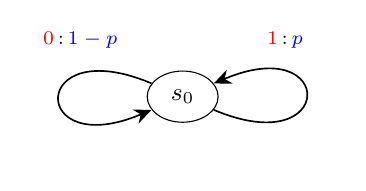
\begin{tikzpicture}
  \node[st] (s0) {$s_0$};
  \draw[tr] (s0) to[out=157,in=203,looseness=13] (s0);
  \draw[tr] (s0) to[out=-23,in=23,looseness=13]  (s0);
  \node[el] at (-1.30,0.72) {\eL{0}{1-p}};
  \node[el] at ( 1.30,0.72) {\eL{1}{p}};
\end{tikzpicture}}

% ---------------------------------------------------------------------
%  zero-one-random.  Example 2, and again as the reduction of Example 4.
%    T^(0): s0 -> s1 = 1,  sR -> s0 = 1-p
%    T^(1): s1 -> sR = 1,  sR -> s0 = p
%  #1 prefixes the node names, so the reduction can share one picture
%  with Example 4 without the two machines' s0/s1/sR colliding.
% ---------------------------------------------------------------------
\newcommand{\zorgraph}[1]{%
  \node[st] (#1s0) at (0,0)        {$s_0$};
  \node[st] (#1sR) at (3.3,0)      {$s_R$};
  \node[st] (#1s1) at (1.65,-1.85) {$s_1$};
  \draw[tr] (#1s0) -- node[el, below left]  {\eL{0}{1}}   (#1s1);
  \draw[tr] (#1s1) -- node[el, below right] {\eL{1}{1}}   (#1sR);
  \draw[tr] (#1sR) to[bend right=32] node[el, above] {\eL{1}{p}}   (#1s0);
  \draw[tr] (#1sR) to[bend left=15]  node[el, below] {\eL{0}{1-p}} (#1s0);
}

\newcommand{\figExTwoZOR}{%
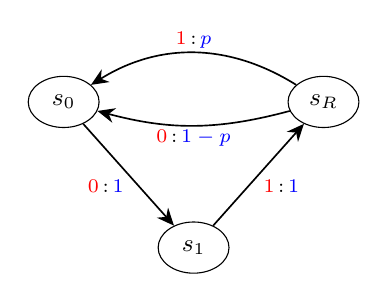
\begin{tikzpicture}\zorgraph{}\end{tikzpicture}}

% ---------------------------------------------------------------------
%  Example 3 -- random-random-XOR.
%    T^(0): so -> s0 = 1-p,  s0 -> sF = 1-q,  s1 -> sT = 1-q,  sF -> so = 1
%    T^(1): so -> s1 = p,    s0 -> sT = q,    s1 -> sF = q,    sT -> so = 1
% ---------------------------------------------------------------------
\newcommand{\figExThreeRRXOR}{%
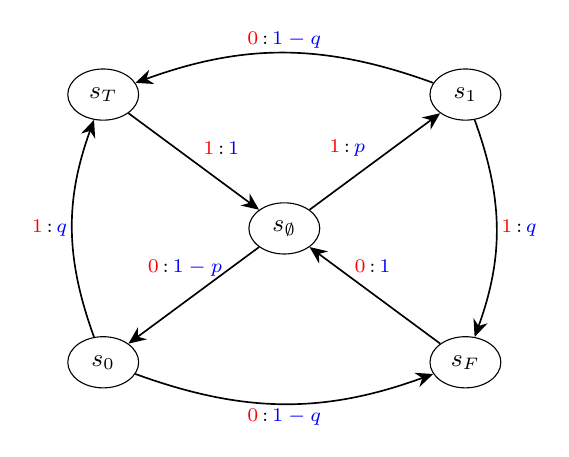
\begin{tikzpicture}
  \node[st] (sT) at (-2.3, 1.70) {$s_T$};
  \node[st] (s1) at ( 2.3, 1.70) {$s_1$};
  \node[st] (se) at ( 0.0, 0.00) {$s_\emptyset$};
  \node[st] (s0) at (-2.3,-1.70) {$s_0$};
  \node[st] (sF) at ( 2.3,-1.70) {$s_F$};
  % rim
  \draw[tr] (s1) to[bend right=20] node[el, above] {\eL{0}{1-q}} (sT);
  \draw[tr] (s1) to[bend left=20]  node[el, right] {\eL{1}{q}}   (sF);
  \draw[tr] (s0) to[bend left=20]  node[el, left]  {\eL{1}{q}}   (sT);
  \draw[tr] (s0) to[bend right=20] node[el, below] {\eL{0}{1-q}} (sF);
  % spokes
  \draw[tr] (sT) -- (se);
  \draw[tr] (se) -- (s1);
  \draw[tr] (se) -- (s0);
  \draw[tr] (sF) -- (se);
  \node[el] at (-0.80, 1.02) {\eL{1}{1}};
  \node[el] at ( 0.80, 1.02) {\eL{1}{p}};
  \node[el] at (-1.26,-0.50) {\eL{0}{1-p}};
  \node[el] at ( 1.12,-0.48) {\eL{0}{1}};
\end{tikzpicture}}

% ---------------------------------------------------------------------
%  Example 4.
%    T~^(0): s0 -> s1 = q,  s0 -> s2 = 1-q,  sR -> s0 = 1-p
%    T~^(1): s1 -> sR = 1,  s2 -> sR = 1,    sR -> s0 = p
% ---------------------------------------------------------------------
\newcommand{\exfourgraph}{%
  \node[st] (s2) at ( 0.00, 1.85) {$s_2$};
  \node[st] (s0) at (-2.05, 0.00) {$s_0$};
  \node[st] (sR) at ( 2.05, 0.00) {$s_R$};
  \node[st] (s1) at ( 0.00,-1.85) {$s_1$};
  \draw[tr] (s0) -- node[el, above left]  {\eL{0}{1-q}} (s2);
  \draw[tr] (s2) -- node[el, above right] {\eL{1}{1}}   (sR);
  \draw[tr] (s0) -- node[el, below left]  {\eL{0}{q}}   (s1);
  \draw[tr] (s1) -- node[el, below right] {\eL{1}{1}}   (sR);
  \draw[tr] (sR) to[bend right=22] node[el, above] {\eL{1}{p}}   (s0);
  \draw[tr] (sR) to[bend left=11]  node[el, below] {\eL{0}{1-p}} (s0);
}

\newcommand{\figExFour}{%
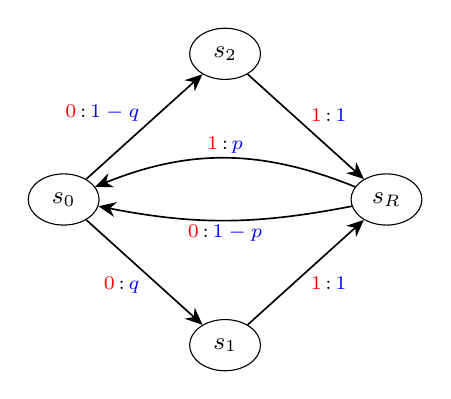
\begin{tikzpicture}\exfourgraph\end{tikzpicture}}

% ---------------------------------------------------------------------
%  Example 4 again, with s2 marked redundant and the machine reduced.
%  The reduction is exactly zero-one-random, hence \zorgraph here too.
% ---------------------------------------------------------------------
\newcommand{\figExFourRedundant}{%
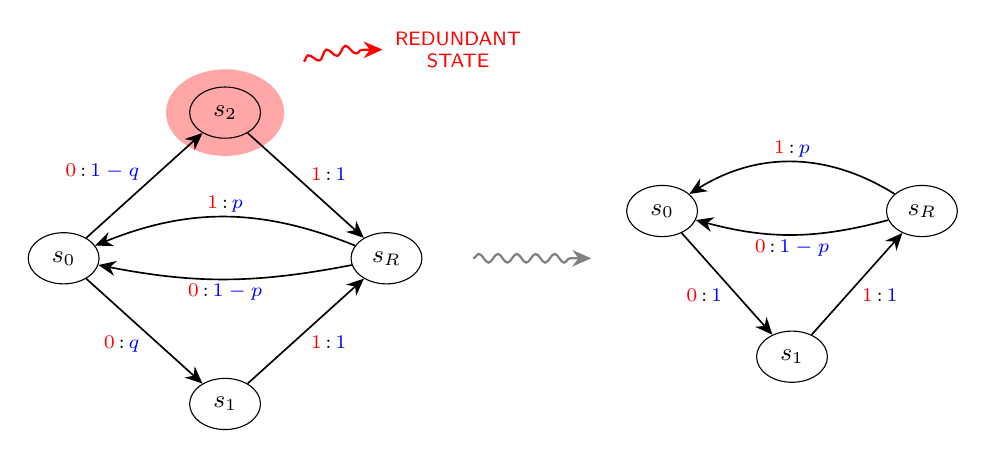
\begin{tikzpicture}
  \exfourgraph
  \begin{scope}[on background layer]
    \node[hl] at (s2) {};
  \end{scope}
  \draw[squig, red] (1.00,2.50) to[out=20,in=180] (2.00,2.65);
  \node[el, red, anchor=west, align=center, font=\scriptsize\sffamily]
        at (2.10,2.65) {REDUNDANT\\STATE};
  \draw[squig] (3.15,0) -- (4.65,0);
  \begin{scope}[shift={(5.55,0.60)}]
    \zorgraph{r}
  \end{scope}
\end{tikzpicture}}

% ---------------------------------------------------------------------
%  Notation.  x and p are variables here, so this one is not coloured.
% ---------------------------------------------------------------------
\newcommand{\figNotation}{%
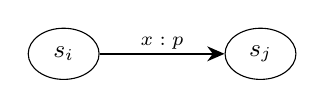
\begin{tikzpicture}[baseline=(si.base)]
  \node[st] (si) at (0,0)   {$s_i$};
  \node[st] (sj) at (2.5,0) {$s_j$};
  \draw[tr] (si) -- node[el, above] {$x : p$} (sj);
\end{tikzpicture}}

% ---------------------------------------------------------------------
%  Minimality -- the same process realised by ever fewer hidden states.
%  The states are deliberately unlabelled in the original: the point is
%  the shrinking state count, not any particular machine.
% ---------------------------------------------------------------------
\newcommand{\figMinimality}{%
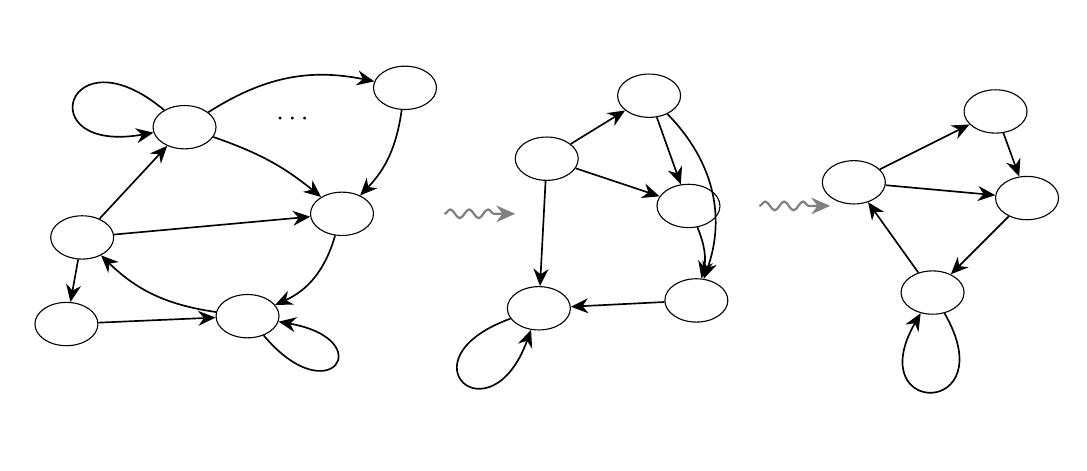
\begin{tikzpicture}[x=1mm, y=1mm]
  % --- six states, with more elided ---
  \begin{scope}
    \node[blob] (a1) at (15,25) {};
    \node[blob] (a2) at (43,30) {};
    \node[blob] (a3) at (35,14) {};
    \node[blob] (a4) at ( 2,11) {};
    \node[blob] (a5) at ( 0, 0) {};
    \node[blob] (a6) at (23, 1) {};
    \node       (ad) at (29,26) {$\cdots$};
    \draw[tr] (a1) to[out=140,in=190,looseness=13] (a1);
    \draw[tr] (a1) to[bend left=22]  (a2);
    \draw[tr] (a1) to[bend left=10]  (a3);
    \draw[tr] (a2) to[bend left=18]  (a3);
    \draw[tr] (a4) -- (a1);
    \draw[tr] (a4) -- (a3);
    \draw[tr] (a4) -- (a5);
    \draw[tr] (a3) to[bend left=25]  (a6);
    \draw[tr] (a5) -- (a6);
    \draw[tr] (a6) to[bend left=18]  (a4);
    \draw[tr] (a6) to[out=-50,in=-10,looseness=13] (a6);
  \end{scope}
  % --- five ---
  \begin{scope}[shift={(60,2)}]
    \node[blob] (b1) at (14,27) {};
    \node[blob] (b2) at ( 1,19) {};
    \node[blob] (b3) at (19,13) {};
    \node[blob] (b4) at ( 0, 0) {};
    \node[blob] (b5) at (20, 1) {};
    \draw[tr] (b2) -- (b1);
    \draw[tr] (b1) -- (b3);
    \draw[tr] (b1) to[bend left=32] (b5);
    \draw[tr] (b2) -- (b3);
    \draw[tr] (b2) -- (b4);
    \draw[tr] (b3) to[bend left=18] (b5);
    \draw[tr] (b5) -- (b4);
    \draw[tr] (b4) to[out=200,in=250,looseness=13] (b4);
  \end{scope}
  % --- four ---
  \begin{scope}[shift={(100,4)}]
    \node[blob] (c1) at (18,23) {};
    \node[blob] (c2) at ( 0,14) {};
    \node[blob] (c3) at (22,12) {};
    \node[blob] (c4) at (10, 0) {};
    \draw[tr] (c2) -- (c1);
    \draw[tr] (c1) -- (c3);
    \draw[tr] (c2) -- (c3);
    \draw[tr] (c3) -- (c4);
    \draw[tr] (c4) -- (c2);
    \draw[tr] (c4) to[out=-60,in=-120,looseness=13] (c4);
  \end{scope}
  % --- and the reductions between them ---
  \draw[squig] (48,14) -- (57,14);
  \draw[squig] (88,15) -- (97,15);
\end{tikzpicture}}


% Underlined emphasis, matching the underlining in the handwritten original.
% (ulem is not installed here; \underline is fine for these short phrases.)
\newcommand{\uw}[1]{\underline{\smash{#1}}}

% Slide titles in the original are underlined by hand.
\setbeamertemplate{frametitle}{%
  \vskip0.6em%
  \underline{\insertframetitle}\par\vskip0.2em%
}

% --- transcription helpers -------------------------------------------
% Highlighter pens used in the original to pair factors across two
% consecutive expressions (slides 6, 12, 15).
\definecolor{hly}{RGB}{253,246,124}
\definecolor{hlg}{RGB}{150,235,150}
\definecolor{hlc}{RGB}{142,233,246}
\definecolor{hlo}{RGB}{250,206,152}
\definecolor{hlr}{RGB}{248,132,132}
\newcommand{\py}[1]{\colorbox{hly}{\ensuremath{#1}}}
\newcommand{\pg}[1]{\colorbox{hlg}{\ensuremath{#1}}}
\newcommand{\pc}[1]{\colorbox{hlc}{\ensuremath{#1}}}
\newcommand{\po}[1]{\colorbox{hlo}{\ensuremath{#1}}}
\newcommand{\pr}[1]{\colorbox{hlr}{\ensuremath{#1}}}

% "think" squiggle used on the definition slide.
\newcommand{\think}{\overset{\text{\tiny ``think''}}{\rightsquigarrow}}

% Fixed-width cells so that the grey row/column state labels line up
% with the matrix entries, as they do in the handwritten original.
\newcommand{\ec}[1]{\makebox[2.15em]{\ensuremath{#1}}}          % entry
\newcommand{\lc}[1]{\makebox[2.15em]{\ensuremath{\scriptstyle\color{black!55}#1}}} % label
\newcommand{\ecs}[1]{\makebox[1.85em]{\ensuremath{\scriptstyle#1}}}
\newcommand{\lcs}[1]{\makebox[1.85em]{\ensuremath{\scriptscriptstyle\color{black!55}#1}}}

% The all-ones column vector.
% NOTE: amssymb provides no blackboard-bold digits -- \mathbb{1} silently
% renders as \oint. bbm / bbold / dsfont are not installed here, so the
% double-struck 1 is composed by hand. If you compile somewhere with bbm
% available, replace the body with \mathbbm{1}.
\newcommand{\ones}{\ensuremath{\mathrm{1}\mkern-6mu\mathrm{1}}}

\title{Computational Mechanics}
\date{ILIAD Intensive --- Spring 2026}
\author{}

\begin{document}

% ---------------------------------------------------------------- 1 ---
\begin{frame}[plain]
  \vfill
  \begin{center}
    {\LARGE \underline{Computational Mechanics:}}\\[2em]
    {\LARGE 1. Overview \& Scope}\\[4em]
    {\large ILIAD INTENSIVE --- SPRING 2026}
  \end{center}
  \vfill
\end{frame}

% ---------------------------------------------------------------- 2 ---
\begin{frame}{Outline:}
  \vspace{1em}
  \begin{enumerate}
    \item What is Computational Mechanics?
    \item Computational Mechanics \& AI Safety
    \item Overview --- where is the program at?
    \item Scope --- what will we tackle today?
  \end{enumerate}
\end{frame}

% ---------------------------------------------------------------- 3 ---
\begin{frame}{What is Computational Mechanics?}
  \begin{itemize}
    \item[\textasteriskcentered] \uw{Statistical Mechanics} makes predictions about the
          behaviour of systems by considering their \uw{statistical} properties. E.g.
  \end{itemize}
  \begin{center}
    
\includegraphics[width=0.86\textwidth]{statmech}
  \end{center}
  \begin{itemize}
    \item[\textasteriskcentered] \uw{Computational Mechanics} (comp-mech) makes predictions
          about the behaviour of systems by considering their \uw{computational} properties. E.g.
  \end{itemize}
  \begin{center}
    
\includegraphics[width=0.72\textwidth]{compmech}
  \end{center}
\end{frame}

% ---------------------------------------------------------------- 4 ---
\begin{frame}{What is Computational Mechanics?}
  \vspace{0.5em}
  Some questions that are central to comp-mech:
  \vspace{0.8em}
  \begin{itemize}
    \item[\textasteriskcentered] How much of the past does a system store?
    \vspace{0.4em}
    \item[\textasteriskcentered] How does the system store this information?
    \vspace{0.4em}
    \item[\textasteriskcentered] How does this information affect system behaviour?
  \end{itemize}
  \vspace{1em}
  We will consider each of these questions for transformers today!
\end{frame}

% ---------------------------------------------------------------- 5 ---
\begin{frame}{What is Computational Mechanics?}
  \vspace{0.5em}
  Not all systems are interesting! Comp-mech places an emphasis on those
  performing \uw{optimal prediction}. In this setting the central question becomes:
  \vspace{1em}
  \begin{center}
    \begin{tcolorbox}[width=0.8\textwidth,colback=blue!8,colframe=blue!55,
                      boxrule=0.8pt,arc=1pt,halign=center]
      What are convergent structures relevant for\\ optimal prediction?
    \end{tcolorbox}
  \end{center}
  \vspace{1em}
  Insight on this question greatly constrains our search space when
  considering \uw{optimal predictors}.
\end{frame}

% ---------------------------------------------------------------- 6 ---
\begin{frame}{Computational Mechanics \& AI Safety}
  \vspace{0.3em}
  We have strong reason to believe that AI systems will pursue a range of
  \uw{instrumental goals} in service of their \uw{terminal goal}
  \begin{center}
    
\includegraphics[height=0.58\textheight]{instrumental}
  \end{center}
\end{frame}

% ---------------------------------------------------------------- 7 ---
\begin{frame}{Computational Mechanics \& AI Safety}
  \vspace{0.3em}
  Comp-mech uses an \uw{instrumental goal} as an intervention target point
  \begin{center}
    
\includegraphics[height=0.5\textheight]{intervention}
  \end{center}
  By considering internal representations consistent with optimal
  prediction the search space is reduced.
\end{frame}

% ---------------------------------------------------------------- 8 ---
\begin{frame}{Computational Mechanics \& AI Safety}
  \vspace{0.3em}
  Targeting an instrumental goal is \uw{scale-free} --- it will be relevant
  to current and future models
  \begin{center}
    
\includegraphics[width=0.92\textwidth]{capability_scale}
  \end{center}
  \vspace{0.3em}
  Which contrasts \uw{scale-sensitive} approaches e.g.\ AI control that are
  only applicable up to a fixed capability scale.
  \vspace{0.5em}

  Moreover, as capabilities increase models will better approximate
  \uw{optimal predictors}.
\end{frame}

% ---------------------------------------------------------------- 9 ---
\begin{frame}{Overview --- where is the program at?}
  \vspace{0.5em}
  Comp-mech applied to AI safety is a young research program
  ($\sim$2 years). There is much to do!
  \vspace{1em}

  Progress can be broken down into two orthogonal directions:
  \vspace{0.8em}
  \begin{itemize}
    \item[\textasteriskcentered] For what classes of data generating \uw{processes}
          do we understand optimal prediction?
    \vspace{0.5em}
    \item[\textasteriskcentered] For what scale of \uw{neural networks} have we
          identified the structures of optimal prediction?
  \end{itemize}
\end{frame}

% --------------------------------------------------------------- 10 ---
\begin{frame}{Processes:}
  \vspace{0.3em}
  Fix a (computable) stochastic process and consider:
  \vspace{0.4em}

  What resources are required to generate this process?
  \vspace{0.4em}

  This naturally leads to a hierarchy:
  \begin{center}
    \includegraphics[height=0.56\textheight]{hierarchy}
  \end{center}
\end{frame}

% --------------------------------------------------------------- 11 ---
\begin{frame}{Processes:}
  \vspace{0.3em}
  For what classes of data generating \uw{processes} do we understand
  optimal prediction?
  \begin{center}
    \includegraphics[height=0.58\textheight]{hierarchy_green}
  \end{center}
\end{frame}

% --------------------------------------------------------------- 12 ---
\begin{frame}{Neural Networks:}
  \vspace{0.3em}
  For what scale of \uw{neural networks} have we identified the structures
  of optimal prediction?
  \vspace{0.8em}
  \begin{itemize}
    \item[\textasteriskcentered] Transformer: $\sim 10^{5}$ parameters
    \vspace{0.3em}
    \item[\textasteriskcentered] LSTM: $\sim 10^{5}$ parameters
    \vspace{0.3em}
    \item[\textasteriskcentered] RNN: $\sim 10^{4}$ parameters
    \vspace{0.3em}
    \item[\textasteriskcentered] GRU: $\sim 10^{5}$ parameters
  \end{itemize}
  \vspace{1em}
  Very toy compared to current frontier models ($\sim 10^{12}$)!
\end{frame}

% --------------------------------------------------------------- 13 ---
\begin{frame}{Overview --- where is the program at?}
  \vspace{0.3em}
  We are working to push the Pareto frontier:
  \begin{center}
    \includegraphics[height=0.66\textheight]{pareto}
  \end{center}
\end{frame}

% --------------------------------------------------------------- 14 ---
% Same slide as 13, with the "Wild Speculation" note overlaid on the plot.
\begin{frame}{Overview --- where is the program at?}
  \vspace{0.3em}
  We are working to push the Pareto frontier:
  \begin{center}
    \includegraphics[height=0.66\textheight]{pareto}
  \end{center}
  \vspace{-0.60\textheight}
  \begin{tcolorbox}[colback=yellow!6,colframe=black!25,boxrule=0.6pt,arc=2pt]
    {\color{red}\underline{\textbf{Wild Speculation:}}}
    \vspace{0.6em}

    As the research program is scale-free one view is that we should
    develop the foundations such that future automated AI Safety
    researchers can pursue these ideas independently
  \end{tcolorbox}
\end{frame}

% --------------------------------------------------------------- 15 ---
\begin{frame}{Scope --- what will we tackle today?}
  \vspace{0.3em}
  We will take a slightly narrower view and consider:
  \begin{center}
    \includegraphics[height=0.68\textheight]{scope}
  \end{center}
\end{frame}

% --------------------------------------------------------------- 16 ---
\begin{frame}{Plan:}
  \vspace{0.8em}
  \begin{enumerate}
    \item Foundations --- Hidden Markov Models \hfill [lecture/exercises]
    \vspace{0.4em}
    \item Foundations --- Prediction \hfill [lecture/exercises]
    \vspace{0.4em}
    \item Applications --- Designing Processes \hfill [tutorial]
    \vspace{0.4em}
    \item Applications --- Belief geometry in transformers \hfill [reading]
    \vspace{0.4em}
    \item Applications --- How do transformers do it? \hfill [tutorial]
    \vspace{0.4em}
    \item Q\,\&\,A with Adam Shai and/or Paul Riechers
  \end{enumerate}
\end{frame}

% --------------------------------------------------------------- 17 ---
\begin{frame}[plain]
  \vfill
  \begin{center}
    {\Huge \underline{Questions?}}
  \end{center}
  \vfill
\end{frame}

% ---------------------------------------------------------------- 1 ---
\begin{frame}[plain]
  \vfill
  \begin{center}
    {\LARGE \underline{Computational Mechanics:}}\\[2em]
    {\LARGE 2. Hidden Markov Models}\\[4em]
    {\large ILIAD INTENSIVE --- SPRING 2026}
  \end{center}
  \vfill
\end{frame}

% ---------------------------------------------------------------- 2 ---
\begin{frame}{Outline:}
  \vspace{1em}
  \begin{enumerate}
    \item What is a hidden Markov Model (HMM)?
    \vspace{0.4em}
    \item HMM minimality \& uniqueness
    \vspace{0.4em}
    \item Generalised hidden Markov Model (GHMM)
  \end{enumerate}
\end{frame}

% ---------------------------------------------------------------- 3 ---
\begin{frame}{What is a hidden Markov Model?}
  \vspace{0.3em}
  Intuitively, a hidden Markov Model (HMM) is a stochastic process that
  consists of two components:
  \vspace{0.8em}
  \begin{itemize}
    \item[\textasteriskcentered] A \uw{`hidden'} unobserved component that evolves
          according to a \uw{Markovian} dynamic --- the next hidden state only
          depends on the current hidden state.
    \vspace{0.6em}
    \item[\textasteriskcentered] An observed component that depends only on the
          current hidden state in a possibly lossy way.
  \end{itemize}
\end{frame}

% ---------------------------------------------------------------- 4 ---
% Plato's cave. The blue/red labels are part of the cropped figure.
\begin{frame}{What is a hidden Markov Model?}
  \begin{center}
    
\includegraphics[height=0.74\textheight]{cave}
  \end{center}
\end{frame}

% ---------------------------------------------------------------- 5 ---
\begin{frame}{What is a hidden Markov Model?}
  \vspace{0.2em}
  A (Mealy-type) HMM consists of:
  \vspace{0.5em}
  \begin{itemize}
    \item[\textasteriskcentered] A set $S$ \quad $\think$ \quad collection of hidden states
    \vspace{0.3em}
    \item[\textasteriskcentered] A set $\mathcal{X}$ \quad $\think$ \quad vocabulary of observations
    \vspace{0.3em}
    \item[\textasteriskcentered] A collection of transition matrices
          $(T^{(x)})_{x\in\mathcal{X}}$
          \hfill
          {\scriptsize $\think$
           \begin{tabular}{@{}l@{}}dynamic that determines\\
                                   emissions \& hidden\\
                                   state transitions\end{tabular}}
  \end{itemize}
  \vspace{0.2em}
  \[
    \text{where}\quad
    T^{(x)}_{ij} := P\!\left(X=x,\ S_j=s_j \mid S_i=s_i\right)
                  = P\!\left(x,\ s_j \mid s_i\right)
  \]
  \vspace{-0.4em}

  It is convenient to use the following graphical notation to visualise
  process transitions:
  \begin{center}
    \figNotation
    \hspace{3em}
    $p = P(x,\ s_j \mid s_i)$
  \end{center}
\end{frame}

% ---------------------------------------------------------------- 6 ---
% No frame title in the original.
\begin{frame}
  \vspace{0.5em}
  Fix an initial distribution over hidden states
  \[
    \eta^{(\emptyset)}_i := \big(P(s_i)\big)_i\ ,
    \qquad i = 1,\ldots,|S|
  \]
  The probability of observing the sequence of emissions
  $w := w_1 w_2 \cdots w_n \in \mathcal{X}^n$ factorises as:
  \[
    P(w) = \sum_{s_0,\ldots,s_n}
      \py{P(s_0)}\,
      \pg{P(w_1,s_1|s_0)}\,
      \pc{P(w_2,s_2|s_1)} \cdots
      \po{P(w_n,s_n|s_{n-1})}
  \]
  Conveniently, the above expression can be stated in terms of HMM
  transition matrices as:
  \[
    P(w) = \py{\eta^{(\emptyset)}}\,
           \pg{T^{(w_1)}}\,
           \pc{T^{(w_2)}} \cdots
           \po{T^{(w_n)}}\,
           \pr{\ones}
  \]
  \vspace{-0.6em}
  \[
    \text{where}\quad
    \eta^{(\emptyset)} -
    \text{\footnotesize\begin{tabular}{@{}l@{}}row vector\\ w.r.t ordered\\ basis of $S$\end{tabular}}
    \qquad\&\qquad
    \ones = \begin{bmatrix}1\\1\\\vdots\\1\end{bmatrix}
  \]
\end{frame}

% ---------------------------------------------------------------- 7 ---
\begin{frame}
  \vspace{-0.2em}
  \uw{Example 1}: \quad (Biased coin)
  \begin{columns}[c]
    \begin{column}{0.26\textwidth}
      \[ S = \{s_0\} \]
      \[ \mathcal{X} = \{{\color{red}0},{\color{red}1}\} \]
    \end{column}
    \begin{column}{0.36\textwidth}
      \begin{center}\scalebox{0.80}{\figExOneCoin}\end{center}
    \end{column}
    \begin{column}{0.30\textwidth}
      \[ T^{({\color{red}0})} = {\color{blue}1-p} \]
      \[ T^{({\color{red}1})} = {\color{blue}p} \]
    \end{column}
  \end{columns}

  \vspace{0.2em}
  \uw{Example 2}: \quad (zero-one-random)
  \begin{columns}[c]
    \begin{column}{0.26\textwidth}
      \[ S = \{s_0,s_1,s_R\} \]
      \[ \mathcal{X} = \{{\color{red}0},{\color{red}1}\} \]
    \end{column}
    \begin{column}{0.30\textwidth}
      \begin{center}\scalebox{0.72}{\figExTwoZOR}\end{center}
    \end{column}
    \begin{column}{0.38\textwidth}
      \[
        T^{({\color{red}0})} =
        \begin{array}{@{}c@{}}
          \begin{array}{@{}c@{}c@{}c@{}}\lc{s_0}&\lc{s_1}&\lc{s_R}\end{array}\\[0.1em]
          \left[\begin{array}{@{}c@{}c@{}c@{}}
            \ec{0} & \ec{\color{blue}1} & \ec{0}\\
            \ec{0} & \ec{0} & \ec{0}\\
            \ec{\color{blue}1-p} & \ec{0} & \ec{0}
          \end{array}\right]
        \end{array}
        \begin{array}{@{}l@{}}\\[0.1em]\lc{s_0}\\ \lc{s_1}\\ \lc{s_R}\end{array}
      \]
      \vspace{-0.8em}
      \[
        T^{({\color{red}1})} =
        \left[\begin{array}{@{}c@{}c@{}c@{}}
          \ec{0} & \ec{0} & \ec{0}\\
          \ec{0} & \ec{0} & \ec{\color{blue}1}\\
          \ec{\color{blue}p} & \ec{0} & \ec{0}
        \end{array}\right]
      \]
    \end{column}
  \end{columns}

  \vspace{0.1em}
  \hspace{1.5em}$\ldots\,0\,1\,R\,0\,1\ldots$
  \hspace{2em} $R \in \{0,1\}$
\end{frame}

% ---------------------------------------------------------------- 8 ---
\begin{frame}
  \vspace{0.2em}
  \uw{Example 3}: \quad (random--random--XOR)
  \begin{columns}[c]
    \begin{column}{0.36\textwidth}
      \[ S = \{s_\emptyset,s_0,s_1,s_F,s_T\} \]
      \[ \mathcal{X} = \{{\color{red}0},{\color{red}1}\} \]
    \end{column}
    \begin{column}{0.60\textwidth}
      \begin{center}\scalebox{0.72}{\figExThreeRRXOR}\end{center}
    \end{column}
  \end{columns}

  \vspace{0.0em}
  \begin{columns}[c]
    \begin{column}{0.49\textwidth}
      \[
        T^{({\color{red}0})} =
        \begin{array}{@{}c@{}}
          \begin{array}{@{}c@{}c@{}c@{}c@{}c@{}}
            \lcs{s_\emptyset}&\lcs{s_0}&\lcs{s_1}&\lcs{s_F}&\lcs{s_T}\end{array}\\[0.1em]
          \left[\begin{array}{@{}c@{}c@{}c@{}c@{}c@{}}
            \ecs{0}&\ecs{\color{blue}1-p}&\ecs{0}&\ecs{0}&\ecs{0}\\
            \ecs{0}&\ecs{0}&\ecs{0}&\ecs{\color{blue}1-q}&\ecs{0}\\
            \ecs{0}&\ecs{0}&\ecs{0}&\ecs{0}&\ecs{\color{blue}1-q}\\
            \ecs{1}&\ecs{0}&\ecs{0}&\ecs{0}&\ecs{0}\\
            \ecs{0}&\ecs{0}&\ecs{0}&\ecs{0}&\ecs{0}
          \end{array}\right]
        \end{array}
        \begin{array}{@{}l@{}}\\[0.1em]
          \lcs{s_\emptyset}\\ \lcs{s_0}\\ \lcs{s_1}\\ \lcs{s_F}\\ \lcs{s_T}\end{array}
      \]
    \end{column}
    \begin{column}{0.49\textwidth}
      \[
        T^{({\color{red}1})} =
        \left[\begin{array}{@{}c@{}c@{}c@{}c@{}c@{}}
          \ecs{0}&\ecs{0}&\ecs{\color{blue}p}&\ecs{0}&\ecs{0}\\
          \ecs{0}&\ecs{0}&\ecs{0}&\ecs{0}&\ecs{\color{blue}q}\\
          \ecs{0}&\ecs{0}&\ecs{0}&\ecs{\color{blue}q}&\ecs{0}\\
          \ecs{0}&\ecs{0}&\ecs{0}&\ecs{0}&\ecs{0}\\
          \ecs{1}&\ecs{0}&\ecs{0}&\ecs{0}&\ecs{0}
        \end{array}\right]
      \]
    \end{column}
  \end{columns}
\end{frame}

% ---------------------------------------------------------------- 9 ---
\begin{frame}
  \vspace{0.2em}
  \uw{Example 4}:
  \begin{columns}[c]
    \begin{column}{0.42\textwidth}
      \[ S = \{s_0,s_1,s_2,s_R\} \]
      \[ \mathcal{X} = \{{\color{red}0},{\color{red}1}\} \]
    \end{column}
    \begin{column}{0.52\textwidth}
      \begin{center}\scalebox{0.68}{\figExFour}\end{center}
    \end{column}
  \end{columns}

  \vspace{0.1em}
  \begin{columns}[c]
    \begin{column}{0.49\textwidth}
      \[
        \widetilde{T}^{({\color{red}0})} =
        \begin{array}{@{}c@{}}
          \begin{array}{@{}c@{}c@{}c@{}c@{}}
            \lc{s_0}&\lc{s_1}&\lc{s_2}&\lc{s_R}\end{array}\\[0.1em]
          \left[\begin{array}{@{}c@{}c@{}c@{}c@{}}
            \ec{0}&\ec{\color{blue}q}&\ec{\color{blue}1-q}&\ec{0}\\
            \ec{0}&\ec{0}&\ec{0}&\ec{0}\\
            \ec{0}&\ec{0}&\ec{0}&\ec{0}\\
            \ec{\color{blue}1-p}&\ec{0}&\ec{0}&\ec{0}
          \end{array}\right]
        \end{array}
        \begin{array}{@{}l@{}}\\[0.1em]\lc{s_0}\\ \lc{s_1}\\ \lc{s_2}\\ \lc{s_R}\end{array}
      \]
    \end{column}
    \begin{column}{0.49\textwidth}
      \[
        \widetilde{T}^{({\color{red}1})} =
        \left[\begin{array}{@{}c@{}c@{}c@{}c@{}}
          \ec{0}&\ec{0}&\ec{0}&\ec{0}\\
          \ec{0}&\ec{0}&\ec{0}&\ec{\color{blue}1}\\
          \ec{0}&\ec{0}&\ec{0}&\ec{\color{blue}1}\\
          \ec{\color{blue}p}&\ec{0}&\ec{0}&\ec{0}
        \end{array}\right]
      \]
    \end{column}
  \end{columns}
\end{frame}

% --------------------------------------------------------------- 10 ---
% Same slide as 9, with the red callout overlaid.
\begin{frame}
  \vspace{0.2em}
  \uw{Example 4}:
  \begin{columns}[c]
    \begin{column}{0.42\textwidth}
      \[ S = \{s_0,s_1,s_2,s_R\} \]
      \[ \mathcal{X} = \{{\color{red}0},{\color{red}1}\} \]
    \end{column}
    \begin{column}{0.52\textwidth}
      \begin{center}\scalebox{0.68}{\figExFour}\end{center}
    \end{column}
  \end{columns}

  \vspace{0.1em}
  \begin{columns}[c]
    \begin{column}{0.49\textwidth}
      \[
        \widetilde{T}^{({\color{red}0})} =
        \begin{array}{@{}c@{}}
          \begin{array}{@{}c@{}c@{}c@{}c@{}}
            \lc{s_0}&\lc{s_1}&\lc{s_2}&\lc{s_R}\end{array}\\[0.1em]
          \left[\begin{array}{@{}c@{}c@{}c@{}c@{}}
            \ec{0}&\ec{\color{blue}q}&\ec{\color{blue}1-q}&\ec{0}\\
            \ec{0}&\ec{0}&\ec{0}&\ec{0}\\
            \ec{0}&\ec{0}&\ec{0}&\ec{0}\\
            \ec{\color{blue}1-p}&\ec{0}&\ec{0}&\ec{0}
          \end{array}\right]
        \end{array}
        \begin{array}{@{}l@{}}\\[0.1em]\lc{s_0}\\ \lc{s_1}\\ \lc{s_2}\\ \lc{s_R}\end{array}
      \]
    \end{column}
    \begin{column}{0.49\textwidth}
      \[
        \widetilde{T}^{({\color{red}1})} =
        \left[\begin{array}{@{}c@{}c@{}c@{}c@{}}
          \ec{0}&\ec{0}&\ec{0}&\ec{0}\\
          \ec{0}&\ec{0}&\ec{0}&\ec{\color{blue}1}\\
          \ec{0}&\ec{0}&\ec{0}&\ec{\color{blue}1}\\
          \ec{\color{blue}p}&\ec{0}&\ec{0}&\ec{0}
        \end{array}\right]
      \]
    \end{column}
  \end{columns}
  \vspace{-0.62\textheight}
  \begin{center}
  \begin{tcolorbox}[width=0.72\textwidth,colback=yellow!6,colframe=black!25,
                    boxrule=0.6pt,arc=2pt,halign=center]
    {\color{red}\Large Same process as\\[0.4em] zero-one-random!}
  \end{tcolorbox}
  \end{center}
\end{frame}

% --------------------------------------------------------------- 11 ---
% Same slide again, with the redundant state marked and reduced.
\begin{frame}
  \vspace{0.2em}
  \uw{Example 4}:
  \begin{columns}[c]
    \begin{column}{0.32\textwidth}
      \[ S = \{s_0,s_1,s_2,s_R\} \]
      \[ \mathcal{X} = \{{\color{red}0},{\color{red}1}\} \]
    \end{column}
    \begin{column}{0.64\textwidth}
      \begin{center}\scalebox{0.70}{\figExFourRedundant}\end{center}
    \end{column}
  \end{columns}

  \vspace{0.4em}
  \begin{columns}[c]
    \begin{column}{0.49\textwidth}
      \[
        \widetilde{T}^{({\color{red}0})} =
        \begin{array}{@{}c@{}}
          \begin{array}{@{}c@{}c@{}c@{}c@{}}
            \lc{s_0}&\lc{s_1}&\lc{s_2}&\lc{s_R}\end{array}\\[0.1em]
          \left[\begin{array}{@{}c@{}c@{}c@{}c@{}}
            \ec{0}&\ec{\color{blue}q}&\ec{\color{blue}1-q}&\ec{0}\\
            \ec{0}&\ec{0}&\ec{0}&\ec{0}\\
            \ec{0}&\ec{0}&\ec{0}&\ec{0}\\
            \ec{\color{blue}1-p}&\ec{0}&\ec{0}&\ec{0}
          \end{array}\right]
        \end{array}
        \begin{array}{@{}l@{}}\\[0.1em]\lc{s_0}\\ \lc{s_1}\\ \lc{s_2}\\ \lc{s_R}\end{array}
      \]
    \end{column}
    \begin{column}{0.49\textwidth}
      \[
        \widetilde{T}^{({\color{red}1})} =
        \left[\begin{array}{@{}c@{}c@{}c@{}c@{}}
          \ec{0}&\ec{0}&\ec{0}&\ec{0}\\
          \ec{0}&\ec{0}&\ec{0}&\ec{\color{blue}1}\\
          \ec{0}&\ec{0}&\ec{0}&\ec{\color{blue}1}\\
          \ec{\color{blue}p}&\ec{0}&\ec{0}&\ec{0}
        \end{array}\right]
      \]
    \end{column}
  \end{columns}
\end{frame}

% --------------------------------------------------------------- 12 ---
\begin{frame}
  \vspace{0.5em}
  \[
    \begin{aligned}
      \text{Let}\quad & (T^{(x)})_{x\in\mathcal{X}} && - && \text{Z1R}\\
                      & (\widetilde{T}^{(x)})_{x\in\mathcal{X}} && - && \text{Z1R with redundancy}
    \end{aligned}
  \]
  There exist matrices $U$ \& $V$ such that:
  \[
    \widetilde{T}^{(x)} = V\,T^{(x)}\,U
    \qquad\&\qquad
    \mathrm{Id}_{3\times3} = UV
  \]
  \[
    \eta^{(\emptyset)}U - \text{stochastic}
    \qquad\&\qquad
    V\ones - \text{all ones}
  \]
  for all $x \in \{0,1\}$. It follows that
  \[
    \eta^{(\emptyset)}\,T^{(w_1)}T^{(w_2)}\cdots T^{(w_n)}\,\ones
  \]
  \vspace{-1.0em}
  \[
    = \py{\eta^{(\emptyset)}U}\,
      \pg{V T^{(w_1)} U}\,
      \pc{V T^{(w_2)} U} \cdots
      \po{V T^{(w_n)} U}\,
      \pr{V\ones}
  \]
  \vspace{-1.0em}
  \[
    = \py{\widetilde{\eta}^{(\emptyset)}}\,
      \pg{\widetilde{T}^{(w_1)}}\,
      \pc{\widetilde{T}^{(w_2)}} \cdots
      \po{\widetilde{T}^{(w_n)}}\,
      \pr{\widetilde{\ones}}
  \]
\end{frame}

% --------------------------------------------------------------- 13 ---
\begin{frame}{HMM minimality \& uniqueness}
  \vspace{0.3em}
  A given HMM realisation of a stochastic process may be needlessly large
  i.e.\ have more hidden states than necessary.
  \vspace{1em}

  We say that a HMM realisation of a stochastic process is \uw{minimal} if
  there exists no other HMM realisations with fewer hidden states.
  \begin{center}
    \scalebox{0.92}{\figMinimality}
  \end{center}
\end{frame}

% --------------------------------------------------------------- 14 ---
\begin{frame}
  \vspace{0.5em}
  \uw{Claim}: For a stochastic process that admits an HMM realisation, the
  minimal HMM is \uw{not unique}.
  \vspace{0.8em}

  (I.e.\ there does not exist similarity transforms relating the minimal HMMs.)
  \vspace{0.8em}

  This is quite dissatisfying!
  \vspace{0.8em}

  Suppose we trained a transformer on a process whose minimal HMM is not
  unique; what realisation would it learn the details of?
  \vspace{1.2em}

  Can we identify a simple generalisation of HMMs such that uniqueness is
  guaranteed for the more general class?
\end{frame}

% --------------------------------------------------------------- 15 ---
\begin{frame}
  \vspace{0.4em}
  Consider the output distribution of an HMM with
  $(T^{(x)})_{x\in\mathcal{X}}$ \& initial hidden state dist.\
  $\eta^{(\emptyset)}$
  \[
    P(w) = \eta^{(\emptyset)}\,T^{(w_1)}T^{(w_2)}\cdots T^{(w_n)}\,\ones
  \]
  \vspace{-1.0em}
  % In the original each V^{-1}V pair carries a blue underbrace labelled "Id";
  % underbraces cannot span the highlight boxes, so the note is inlined below.
  \[
    = \py{\eta^{(\emptyset)}V^{-1}}\,
      \pg{V T^{(w_1)} V^{-1}}\,
      \pc{V T^{(w_2)} V^{-1}} \cdots
      \po{V T^{(w_n)} V^{-1}}\,
      \pr{V\ones}
  \]
  \vspace{-1.0em}
  \[
    = \py{\check{\eta}^{(\emptyset)}}\,
      \pg{\check{T}^{(w_1)}}\,
      \pc{\check{T}^{(w_2)}} \cdots
      \po{\check{T}^{(w_n)}}\,
      \pr{\check{\ones}}\ ,
    \qquad V \in GL_{|S|}
  \]
  \vspace{-0.6em}
  \[
    \text{where}\quad
    \check{T}^{(x)} = V T^{(x)} V^{-1}
    \ \&\
    \check{\eta}^{(\emptyset)} = \eta^{(\emptyset)}V^{-1}
    \ \&\
    \check{\ones} = V\ones
  \]
  \vspace{-0.4em}

  An identical process is produced by the transition matrices
  $(\check{T}^{(x)})_{x\in\mathcal{X}}$ and the vectors
  $\check{\eta}^{(\emptyset)}$ \& $\check{\ones}$.
  \vspace{0.3em}

  $\implies$ Why constrain the transition matrix to have probabilities as
  matrix elements?
\end{frame}

% --------------------------------------------------------------- 16 ---
\begin{frame}{Generalised hidden Markov Model}
  \vspace{0.2em}
  A generalised hidden Markov Model (GHMM) consists of:
  \vspace{0.4em}
  \begin{itemize}
    \item[\textasteriskcentered] A set $\mathcal{X}$
    \vspace{0.2em}
    \item[\textasteriskcentered] A collection of transition matrices
          $(T^{(x)})_{x\in\mathcal{X}}$
          \ {\color{blue}\small $\rightsquigarrow$ not necessarily sub-stochastic!}
    \vspace{0.2em}
    \item[\textasteriskcentered] An initial row vector $\eta^{(\emptyset)}$
          \ {\color{blue}\small $\rightsquigarrow$ not necessarily stochastic!}
  \end{itemize}
  \vspace{0.3em}
  such that:
  \vspace{0.3em}
  \begin{enumerate}
    \item There exists a (column) vector $\phi$ satisfying:
      \vspace{0.2em}
      \begin{enumerate}
        \item[a)] $T\phi = \phi$ \quad where \quad
                  $\displaystyle T := \sum_{x\in\mathcal{X}} T^{(x)}$
        \vspace{0.3em}
        \item[b)] $\eta^{(\emptyset)}\phi = 1$
      \end{enumerate}
    \vspace{0.4em}
    \item For all $w \in \mathcal{X}^{*}$, \quad
          $\eta^{(\emptyset)}T^{(w_1)}\!\cdots T^{(w_n)}\phi \geq 0$.
  \end{enumerate}
\end{frame}

% --------------------------------------------------------------- 17 ---
\begin{frame}
  \vspace{0.6em}
  The thrust of this definition is to afford additional freedom to
  $(T^{(x)})_{x\in\mathcal{X}}$ and $\eta^{(\emptyset)}$ while maintaining
  the same expression assigning probabilities to emission sequences:
  \[
    P(w) = \eta^{(\emptyset)}\,T^{(w_1)}T^{(w_2)}\cdots T^{(w_n)}\,\phi
  \]
  \vspace{-0.2em}

  (This fact will be explored in the exercises.)
  \vspace{1.4em}

  A consequence of this freedom is that we lose connection to explicit
  hidden states!
\end{frame}

% --------------------------------------------------------------- 18 ---
\begin{frame}
  \vspace{0.3em}
  \uw{Example}: (Bloch Walk)
  \vspace{0.2em}

  Fix $\gamma = \big(2\sqrt{\alpha^{2}+\beta^{2}}\big)^{-1}$, where
  $\alpha > 0$ \& $\beta \in \mathbb{R}$
  \vspace{-0.2em}
  \begin{columns}[c]
    \begin{column}{0.49\textwidth}
      {\small\[
        T^{({\color{red}0})} = \left[\begin{array}{@{}ccc@{}}
          {\color{blue}\tfrac14} & 0 & {\color{blue}2\alpha\beta\gamma^{2}}\\[0.15em]
          0 & {\color{blue}(\alpha^{2}-\beta^{2})\gamma^{2}} & 0\\[0.15em]
          {\color{blue}2\alpha\beta\gamma^{2}} & 0 & {\color{blue}\tfrac14}
        \end{array}\right]
      \]}
    \end{column}
    \begin{column}{0.49\textwidth}
      {\small\[
        T^{({\color{red}1})} = \left[\begin{array}{@{}ccc@{}}
          {\color{blue}\tfrac14} & 0 & {\color{blue}-2\alpha\beta\gamma^{2}}\\[0.15em]
          0 & {\color{blue}(\alpha^{2}-\beta^{2})\gamma^{2}} & 0\\[0.15em]
          {\color{blue}-2\alpha\beta\gamma^{2}} & 0 & {\color{blue}\tfrac14}
        \end{array}\right]
      \]}
    \end{column}
  \end{columns}
  \vspace{0.2em}
  \begin{columns}[c]
    \begin{column}{0.49\textwidth}
      {\small\[
        T^{({\color{red}2})} = \left[\begin{array}{@{}ccc@{}}
          {\color{blue}\tfrac14} & {\color{blue}2\alpha\beta\gamma^{2}} & 0\\[0.15em]
          {\color{blue}2\alpha\beta\gamma^{2}} & {\color{blue}\tfrac14} & 0\\[0.15em]
          0 & 0 & {\color{blue}(\alpha^{2}-\beta^{2})\gamma^{2}}
        \end{array}\right]
      \]}
    \end{column}
    \begin{column}{0.49\textwidth}
      {\small\[
        T^{({\color{red}3})} = \left[\begin{array}{@{}ccc@{}}
          {\color{blue}\tfrac14} & {\color{blue}-2\alpha\beta\gamma^{2}} & 0\\[0.15em]
          {\color{blue}-2\alpha\beta\gamma^{2}} & {\color{blue}\tfrac14} & 0\\[0.15em]
          0 & 0 & {\color{blue}(\alpha^{2}-\beta^{2})\gamma^{2}}
        \end{array}\right]
      \]}
    \end{column}
  \end{columns}
  \vspace{0.2em}
  \[
    \eta^{(\emptyset)} = \begin{bmatrix}{\color{blue}1} & 0 & 0\end{bmatrix}
    \qquad\qquad
    \phi = \begin{bmatrix}{\color{blue}1}\\0\\0\end{bmatrix}
  \]
\end{frame}

% --------------------------------------------------------------- 19 ---
\begin{frame}
  \vspace{0.6em}
  Returning to our initial motivation\ldots
  \vspace{1.2em}

  \uw{Claim} {\color{blue}\small (Upper '97)}: For a stochastic process that
  admits a GHMM realisation, the minimal GHMM is \uw{unique} (up to
  similarity transformation).
  \vspace{1.4em}

  \hspace{1em}$\implies$ Transformers trained on data emitted from a GHMM
  should learn the structure corresponding to the \uw{minimal} GHMM
  \vspace{1.4em}

  We will discuss this `structure' in the next block!
\end{frame}

% --------------------------------------------------------------- 20 ---
\begin{frame}[plain]
  \vfill
  \begin{center}
    {\Huge \underline{Questions?}}
  \end{center}
  \vfill
\end{frame}

\end{document}
